\section*{DAML-S}

\subsection*{Introduction}
The target is to find ways and technologies that will enable us to describe, simulate, automatically compose, test and verify Web service compositions.
For this to work it is necessary to have a way to describe these Semantic Web services. We come to the conclusion that we are in need of a semantic markup language able to describe the content and the capabilities of these web services. The state of the art include languages like OWL we mentioned before. We are going to focus on the DARPA agent markup language (DAML). After the creation of DAML+OIL we improved and created DAML-S. DAML-S is markup language based on DAML+OIL that was created to specifically describe services. Correspondingly, as DAML was replaced with OWL, so DAML-S was also superseded by OWL-S.

\subsection*{DAML+OIL}
DAML+OIL is an AI-inspired description logic-based language for describing taxonomic information. The DAML+OIL is based on top of XML and RDF(S), both defined in the Semantic Web standards. Essentially it is a language with well-defined semantics and a set of language constructs. These include classes, subclasses and properties with domains and ranges. All these can be used to describe a Web domain.

\subsection*{DAML-S}
DAML-S is DAML+OIL ontology for Web services. It is also developed under the auspices of the DAML program. There are few different releases as expected. The DAML-S ontology is able to describe a set of classes and properties, specific to the description of Web services.
It is separated in parts, the upper ontology of DAML-S is created by a service profiler used for describing service advertisements, another process model to enable the description of actual programs that execute each service and a service grounding for describing the transport-level messaging information associated with the actual execution of the program.

\subsection*{DAML-S Examples}
DAML-S process model is able to describe two different types of processes, \emph{atomic} and \emph{composite}. Also it allows the creation a type of \emph{simple} process, which is a description of a view or abstraction of a atomic or composite process to which expands.

\begin{lstlisting}
<daml:Classrdf:ID="Process">
        <daml:unionOfrdf:parseType="daml:collection">
        <daml:Classrdf:about="#AtomicProcess"/>
        <daml:Classrdf:about="#SimpleProcess"/>
        <daml:Classrdf:about="#CompositeProcess"/>
    </daml:unionOf>
</daml:Class>
\end{lstlisting}

An atomic process is a non-decomposable Web-accessible program. It is executed in a single http
call and returns a response. An example of a atomic process is the {\tt LocateBook} that either
returns information about the book or nothing.
\begin{lstlisting}
<daml:Classrdf:ID="LocateBook">
    <rdfs:subClassOf rdf:resource="&process;#AtomicProcess"/>
</daml:Class>
\end{lstlisting}

On the other hand a composite process is composed of other composite or atomic processes. These
composing processes are connected using control constructs, such as \emph{sequence, if-then-else,
while, fork etc}. An example of a composite process is the {\tt Find-n-Buy} service that contains
the LocateBook along with some other services.

\begin{lstlisting}
<daml:Classrdf:ID="CompositeProcess">
    <daml:intersectionOf rdf:parseType="daml:collection">
	<daml:Classrdf:about="#Process"/>
	    <daml:Restrictiondaml:minCardinality="1">
		<daml:onPropertyrdf:resource="#composedOf"/>
	    </daml:Restriction>
    </daml:intersectionOf>
</daml:Class>
\end{lstlisting}

Also, each process is able to has a set of properties, called parameters and can be either be input or output. In the case of the LocateBook an input parameter might be something like the name of the book.

\begin{lstlisting}
<rdf:Propertyrdf:ID="bookName">
    <rdfs:subPropertyOf rdf:resource="&process;#input"/>
    <rdfs:domainrdf:resource="#LocateBook"/>
    <rdfs:rangerdf:resource="&xsd;#string"/>2
</rdf:Property>
\end{lstlisting}

Inputs can be either mandatory or optional. On the other hand, output are usually optional. This is important, in the case of locating and buying a book it is obligatory to provide any type of information about the book but it is optional for an output of type of price, since there is a possibility the book is not found or not currently available. We define this as a conditional class that both describes a condition and an output based on that specific condition.

\begin{lstlisting}
<rdf:Property rdf:ID="output">
    <rdfs:domain rdf:resource="#parameter"/>
    <rdfs:range rdf:resource="#ConditionalOutput"/>
</rdf:Property>
    <daml:Class rdf:ID="ConditionalOutput">
    <daml:subClassOf rdf:resource="http://www.daml.org/...#Thing"/>
    </daml:Class>
    <rdf:Property rdf:ID="coCondition">
    <rdfs:comment>
        The condition of the conditional output.
    </rdfs:comment>
    <rdfs:domain rdf:resource="#ConditionalOutput"/>
    <rdfs:range rdf:resource="#Condition"/>
</rdf:Property>

<rdf:Property rdf:ID="coOutput">
    <rdfs:comment>
        The output of the conditional output.
    </rdfs:comment>
    <rdfs:domain rdf:resource="#ConditionalOutput"/>
    <rdfs:rangerdf:resource="http://www.daml.org/...#Thing"/>
</rdf:Property>
\end{lstlisting}

This offers the ability to the program or function metaphor to be utilized in order to perform real actions in order to create a service. Essentially preconditions for every process is that the process agent has to know in order to execute the process. For example, to execute LocateBook() properly you must execute BookStoreHasBook(bookName). Many web services that are utilized as programs in the web have only preconditions. We analyze further only the abstract preconditions since real physical devices might have more such as bandwidth resources and limited memory.

\subsection*{DAML-S Semantic \& Situation Calculus}

DAML+OIL provides many necessary tools to describe the content and the capabilities of the web. The problem is that DAML+OIL is not able to restrict DAML-S to all and only intended interpretations. The target here is to describe a semantics for that portion of DAML-S that is really relevant to this work, simulation, verification and composition of web services.

The target here is to describe the actual DAML-S in a more expressive language , such as first-order logic. DAML-S is a process modeling language there is a way to transform it to a Process Specification Language(PSL). PSL is a process specification ontology  that can be described in a situation calculus, a first-order logic language for dynamic systems.

\subsection*{Situation Calculus}
The situation calculus language we are going to use is for representing dynamically changing worlds in which all of the changes are the direct results of actions performed by an agent. On the hand, Situations are sequences of actions evolving from a specific situation, called S0. So, if \emph{a} is an action and \emph{s} is a situation then the result of performing \emph{a} in a \emph{s} situation is \emph{do(a,s)}. For example, we can have Own(bookName,s).
Finally, Poss(a,s) is a specific fluent expressing that an action a is possible to perform in a situation s.

Also the notation of Knows($\phi$ ,s) denotes that formula f is a known in a situation s. For example, Knows(Owns("On the road",s)). As a logical step we have Kwhether($\phi$ ,s) = Knows($\phi$ ,s) ∨ Knows($\neg\phi$,s).

Using all this we can create conditional effects and outputs. The conditional effects of an atomic process are represented in the situation calculus as both positive and negative effect axioms of the following form:

\begin{figure}[t]
    \centering
    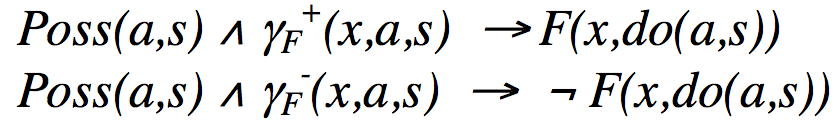
\includegraphics[width=0.5\columnwidth]{daml_cond_effects.png}
    \caption{Conditional effects and outputs}
    \label{fig:Conditional effects and outputs}
\end{figure}

To sum up, the complete situation calculus axiomatization of a DAML-S description includes the sets of axioms described above,
\begin{itemize}
    \item successor state axioms, Dss
    \item action precondition axioms, Dap
    \item foundational axioms of the situation calculus, Σ
    \item axioms describing the initial situation, DS0
    \item unique names for actions, Duna
    \item domain closure axioms for actions, Ddca
\end{itemize}

